
\section{CNN+Attention Implementation}
This section describes the concrete PyTorch implementation of the hybrid CNN+Attention model adapted from Vaswani et al.\ (2017) for time-series classification. The model is defined in \texttt{architectures/cnn\_attention.py} and shares the training, inference, and robustness pipeline with the 1D-CNN and ResNet through the registry in \texttt{model\_selection.py}.

\subsection{Architecture Definition (\texttt{cnn\_attention.py})}
The model has three components: a strided convolutional stem that downsamples and embeds the raw signal, a Transformer encoder that contextualises the embedded sequence, and a CLS-token classifier head.

\subsubsection{Convolutional Stem}
The \texttt{\_ConvStem} module is a sequence of three \texttt{Conv1d $\rightarrow$ GroupNorm(8) $\rightarrow$ ReLU} blocks, each with \textbf{stride 2}. The cumulative stride of 8 reduces the input length from $T = 512$ to $T' = 64$ while expanding the channel count $1 \rightarrow 16 \rightarrow 32 \rightarrow 64$. The kernel sizes shrink progressively from 7 to 5 to 3 as the receptive field grows. The stem serves two purposes:
\begin{itemize}
    \item \textbf{Embedding:} It maps each scalar time step to a 64-dimensional vector, supplying the Transformer with feature vectors rather than raw scalars. Without this, the attention mechanism would be wasted attending between individual noisy points.
    \item \textbf{Quadratic cost reduction:} Self-attention has $\mathcal{O}(T^2 \cdot d)$ complexity. By shrinking the sequence from 512 to 64, the attention cost drops by $(512/64)^2 = 64\times$, making the encoder cheap enough to run at training time.
\end{itemize}
Like the ResNet, the stem uses \texttt{GroupNorm(8)} instead of \texttt{BatchNorm1d}: it has no running statistics, so train and eval normalisation are identical. This was a critical fix --- the baseline implementation used BatchNorm and produced amplitude-dependent predictions at inference, where the same anomaly shape was misclassified if its amplitude was rescaled.

\subsubsection{Sinusoidal Positional Encoding}
\texttt{\_SinusoidalPosEnc} pre-computes the positional encoding table in the constructor and registers it as a non-learnable buffer, then adds it elementwise to the embedded sequence:
\begin{verbatim}
pe[:, 0::2] = torch.sin(position * div_term)
pe[:, 1::2] = torch.cos(position * div_term)
\end{verbatim}
The encoding is added \textit{after} the stem's channel projection so that the embedded feature vectors and the positional codes live in the same 64-dimensional space.

\subsubsection{Transformer Encoder}
The encoder is built from PyTorch's \texttt{nn.TransformerEncoderLayer} with the following configuration:
\begin{itemize}
    \item \textbf{Model dimension:} $d_{\text{model}} = 64$ (matches the stem output).
    \item \textbf{Heads:} $h = 4$, so each head operates on $d_{k} = 16$.
    \item \textbf{Layers:} 2 stacked encoder blocks.
    \item \textbf{Feed-forward dimension:} $d_{\text{ff}} = 4 \cdot d_{\text{model}} = 256$ (the standard 4$\times$ expansion).
    \item \textbf{Activation:} GELU.
    \item \textbf{Normalisation:} Pre-norm (\texttt{norm\_first=True}).
    \item \textbf{Dropout:} 0.1 applied inside the attention and feed-forward sub-layers.
\end{itemize}
The CLS token is a single learnable vector \texttt{nn.Parameter(torch.zeros(1, 1, d\_model))}, initialised with a truncated normal of std 0.02 (the BERT initialisation), and prepended to the embedded sequence before the first encoder layer. After the two encoder layers, the model applies a final \texttt{LayerNorm} and slices out only the CLS position for classification through a \texttt{Linear(64, 7)} head. The total footprint is \textbf{109,655 trainable parameters}.

\subsection{Adaptations Relative to the Reference Implementation}
The reference hybrid model from prior literature used a stem with channels $(32, 64, 64)$, a 4-layer / 8-head / 128-dim Transformer, BatchNorm in the stem, and totalled $\sim$124k parameters. The implementation here makes three deliberate downsizing changes:
\begin{itemize}
    \item \textbf{Narrower stem:} $(32, 64, 64) \rightarrow (16, 32, 64)$, cutting the heaviest part of the network.
    \item \textbf{Smaller Transformer:} 4 layers / 8 heads / 128 dim $\rightarrow$ 2 layers / 4 heads / 64 dim. The synthetic anomaly classes are smooth and morphologically simple --- two encoder layers suffice to mix local features into a class-discriminative CLS representation.
    \item \textbf{GroupNorm in the stem:} replaces BatchNorm, eliminating the amplitude-dependent inference bias.
\end{itemize}

\subsection{Training and Evaluation}
The model uses the same \texttt{train.py} ecosystem as the other two architectures, with two model-specific hyperparameter overrides: the maximum epoch budget is raised to 150 (the attention layers benefit from longer training) and the initial learning rate is doubled to $2 \times 10^{-3}$ to match the larger parameter count and the well-conditioned pre-norm Transformer.

\subsubsection{Training Results}
The model was trained on the 10M-point synthetic dataset (249,985 windows) on an NVIDIA GeForce RTX 5060 Laptop GPU with CUDA 12.8:
\begin{itemize}
    \item \textbf{Convergence:} 38 epochs, 9 minutes 19 seconds. Learning rate decayed from $2 \times 10^{-3}$ to $1.25 \times 10^{-4}$ across 4 reduction steps.
    \item \textbf{Final losses:} Best validation loss = 0.4879, test loss = 0.5802.
    \item \textbf{Test accuracy:} 82.8\% per-window accuracy (51,757 / 62,485 windows). Event-level accuracy is dramatically higher (100\%, see below) due to overlapping-window accumulation during inference.
\end{itemize}

\begin{figure}[H]
    \centering
    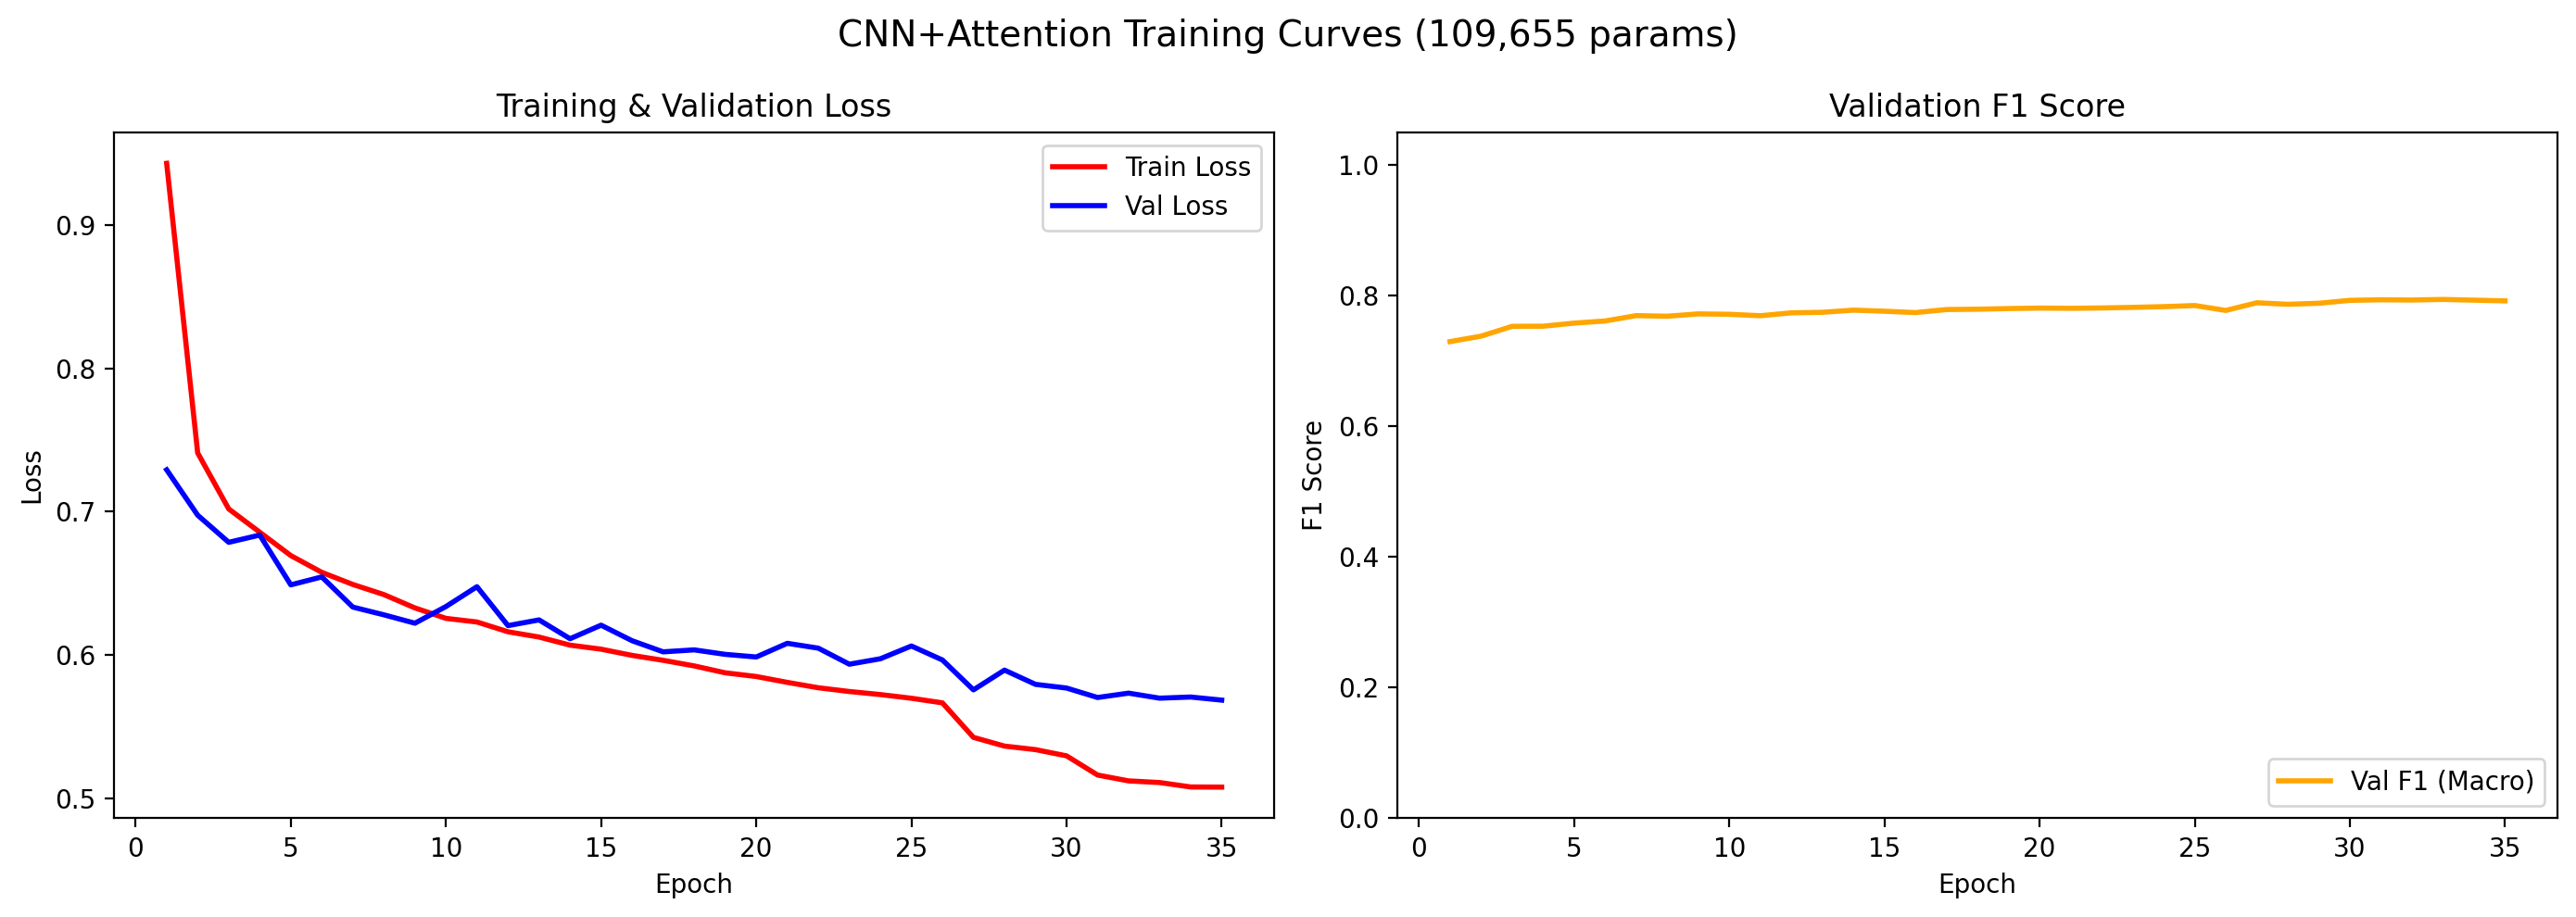
\includegraphics[width=0.7\textwidth]{media/cnn_attention_training_curves.png}
    \caption{CNN+Attention training and validation loss curves. The Transformer's larger parameter count and higher learning rate produce a faster early descent than the 1D-CNN, but the loss plateaus at a higher absolute value because the model is trained on the harder per-window task --- many windows contain a small fraction of anomaly that is impossible to classify without aggregating context across windows.}
    \label{fig:cnn_attention_training_curves}
\end{figure}

\subsubsection{Inference Results}
Inference on the same 100,000-point segment as the ResNet (61 anomaly events), using the dense sliding-window strategy (stride 10, window 512) and softmax accumulation:

\begin{table}[H]
\centering
\caption{CNN+Attention event-level inference results over 61 anomaly events.}
\label{tab:cnn_attention_inference_results}
\small
\begin{tabular}{|l|c|}
\hline
\textbf{Metric} & \textbf{Value} \\
\hline
Total events & 61 \\
\hline
Detection rate (any anomaly) & 100.0\% (61/61) \\
\hline
Exact classification accuracy & 100.0\% (61/61) \\
\hline
Mean confidence & 85.4\% \\
\hline
Inference throughput & 405 windows/sec \\
\hline
Parameters & 109,655 \\
\hline
\end{tabular}
\end{table}

\begin{table}[H]
\centering
\caption{CNN+Attention per-class event-level metrics. The model achieves perfect precision, recall, and F1 across all six anomaly classes.}
\label{tab:cnn_attention_per_class_metrics}
\small
\begin{tabular}{|l|c|c|c|c|}
\hline
\textbf{Class} & \textbf{Support} & \textbf{Precision} & \textbf{Recall} & \textbf{F1-Score} \\
\hline
bell & 13 & 1.000 & 1.000 & 1.000 \\
\hline
bell\_sq & 11 & 1.000 & 1.000 & 1.000 \\
\hline
fast\_ascend & 14 & 1.000 & 1.000 & 1.000 \\
\hline
fast\_descend & 5 & 1.000 & 1.000 & 1.000 \\
\hline
M & 9 & 1.000 & 1.000 & 1.000 \\
\hline
square & 9 & 1.000 & 1.000 & 1.000 \\
\hline
\textbf{Macro Average} & & \textbf{1.000} & \textbf{1.000} & \textbf{1.000} \\
\hline
\end{tabular}
\end{table}

\begin{figure}[H]
    \centering
    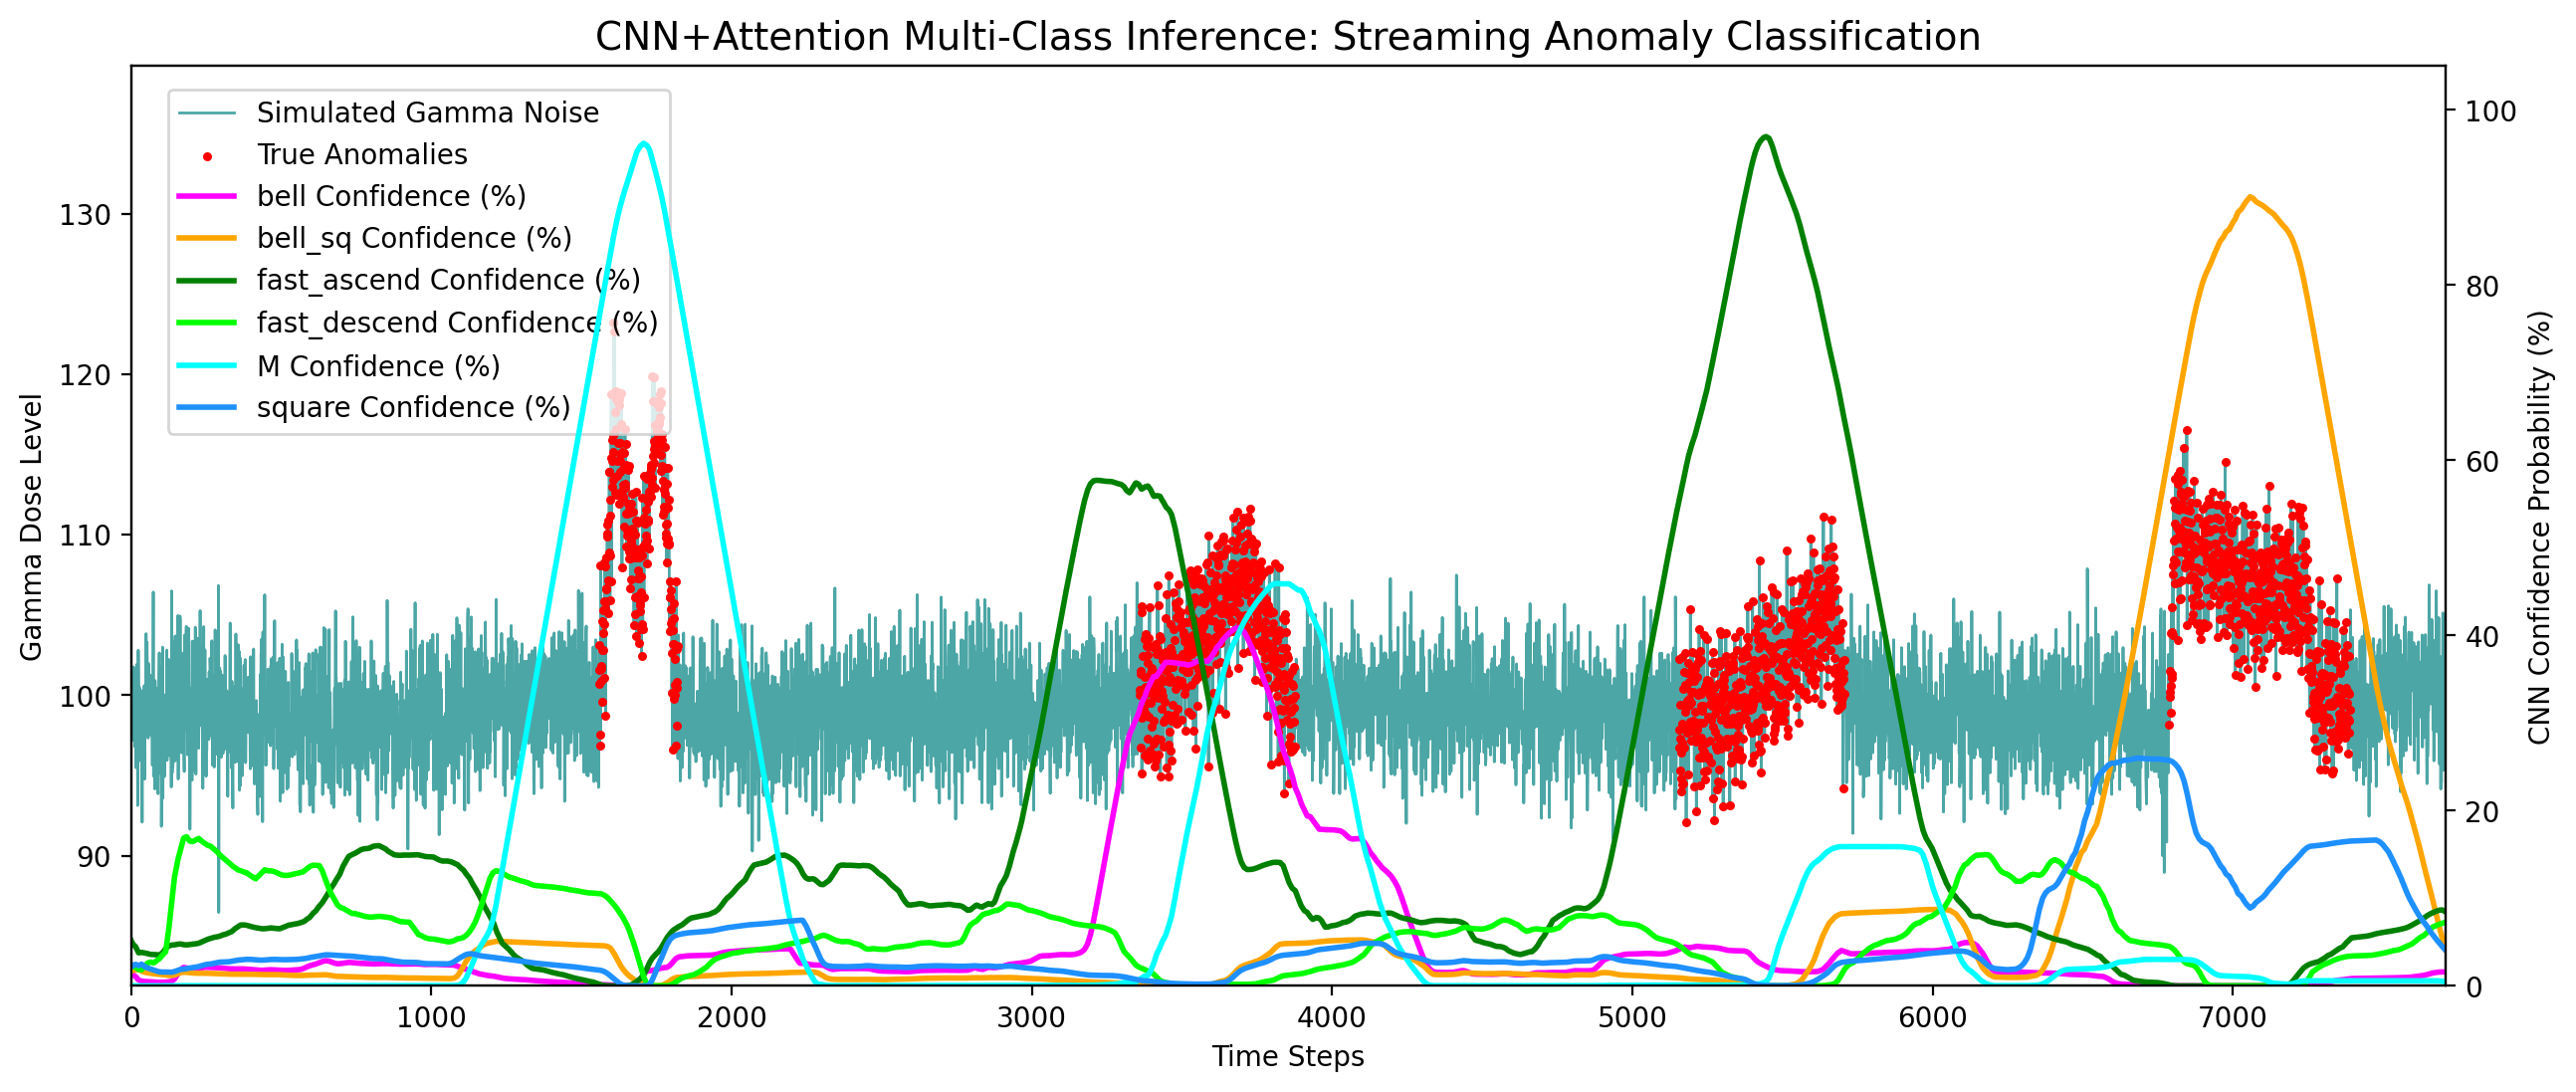
\includegraphics[width=0.7\textwidth]{media/cnn_attention_inference_visualization.png}
    \caption{CNN+Attention per-point class-confidence heatmap overlaid on the simulated gamma dose trace. Compared with the 1D-CNN, the attention-based model produces visibly \emph{wider} confidence plateaus over each anomaly --- the CLS token aggregates information from the entire window, so confidence builds up earlier and decays later than a purely local model.}
    \label{fig:cnn_attention_inference_visualization}
\end{figure}

\subsection{Robustness Analysis (\texttt{robustness\_test.py})}
The hybrid model is exposed to the same two-axis robustness sweep as the 1D-CNN: background noise multiplier from $1\times$ to $3\times$ the baseline $\sigma = 2.70$, and anomaly shape deformation from $1\times$ to $8\times$ the baseline variance 0.04. Each configuration generates a fixed-seed test dataset of 50 events.

\begin{figure}[H]
    \centering
    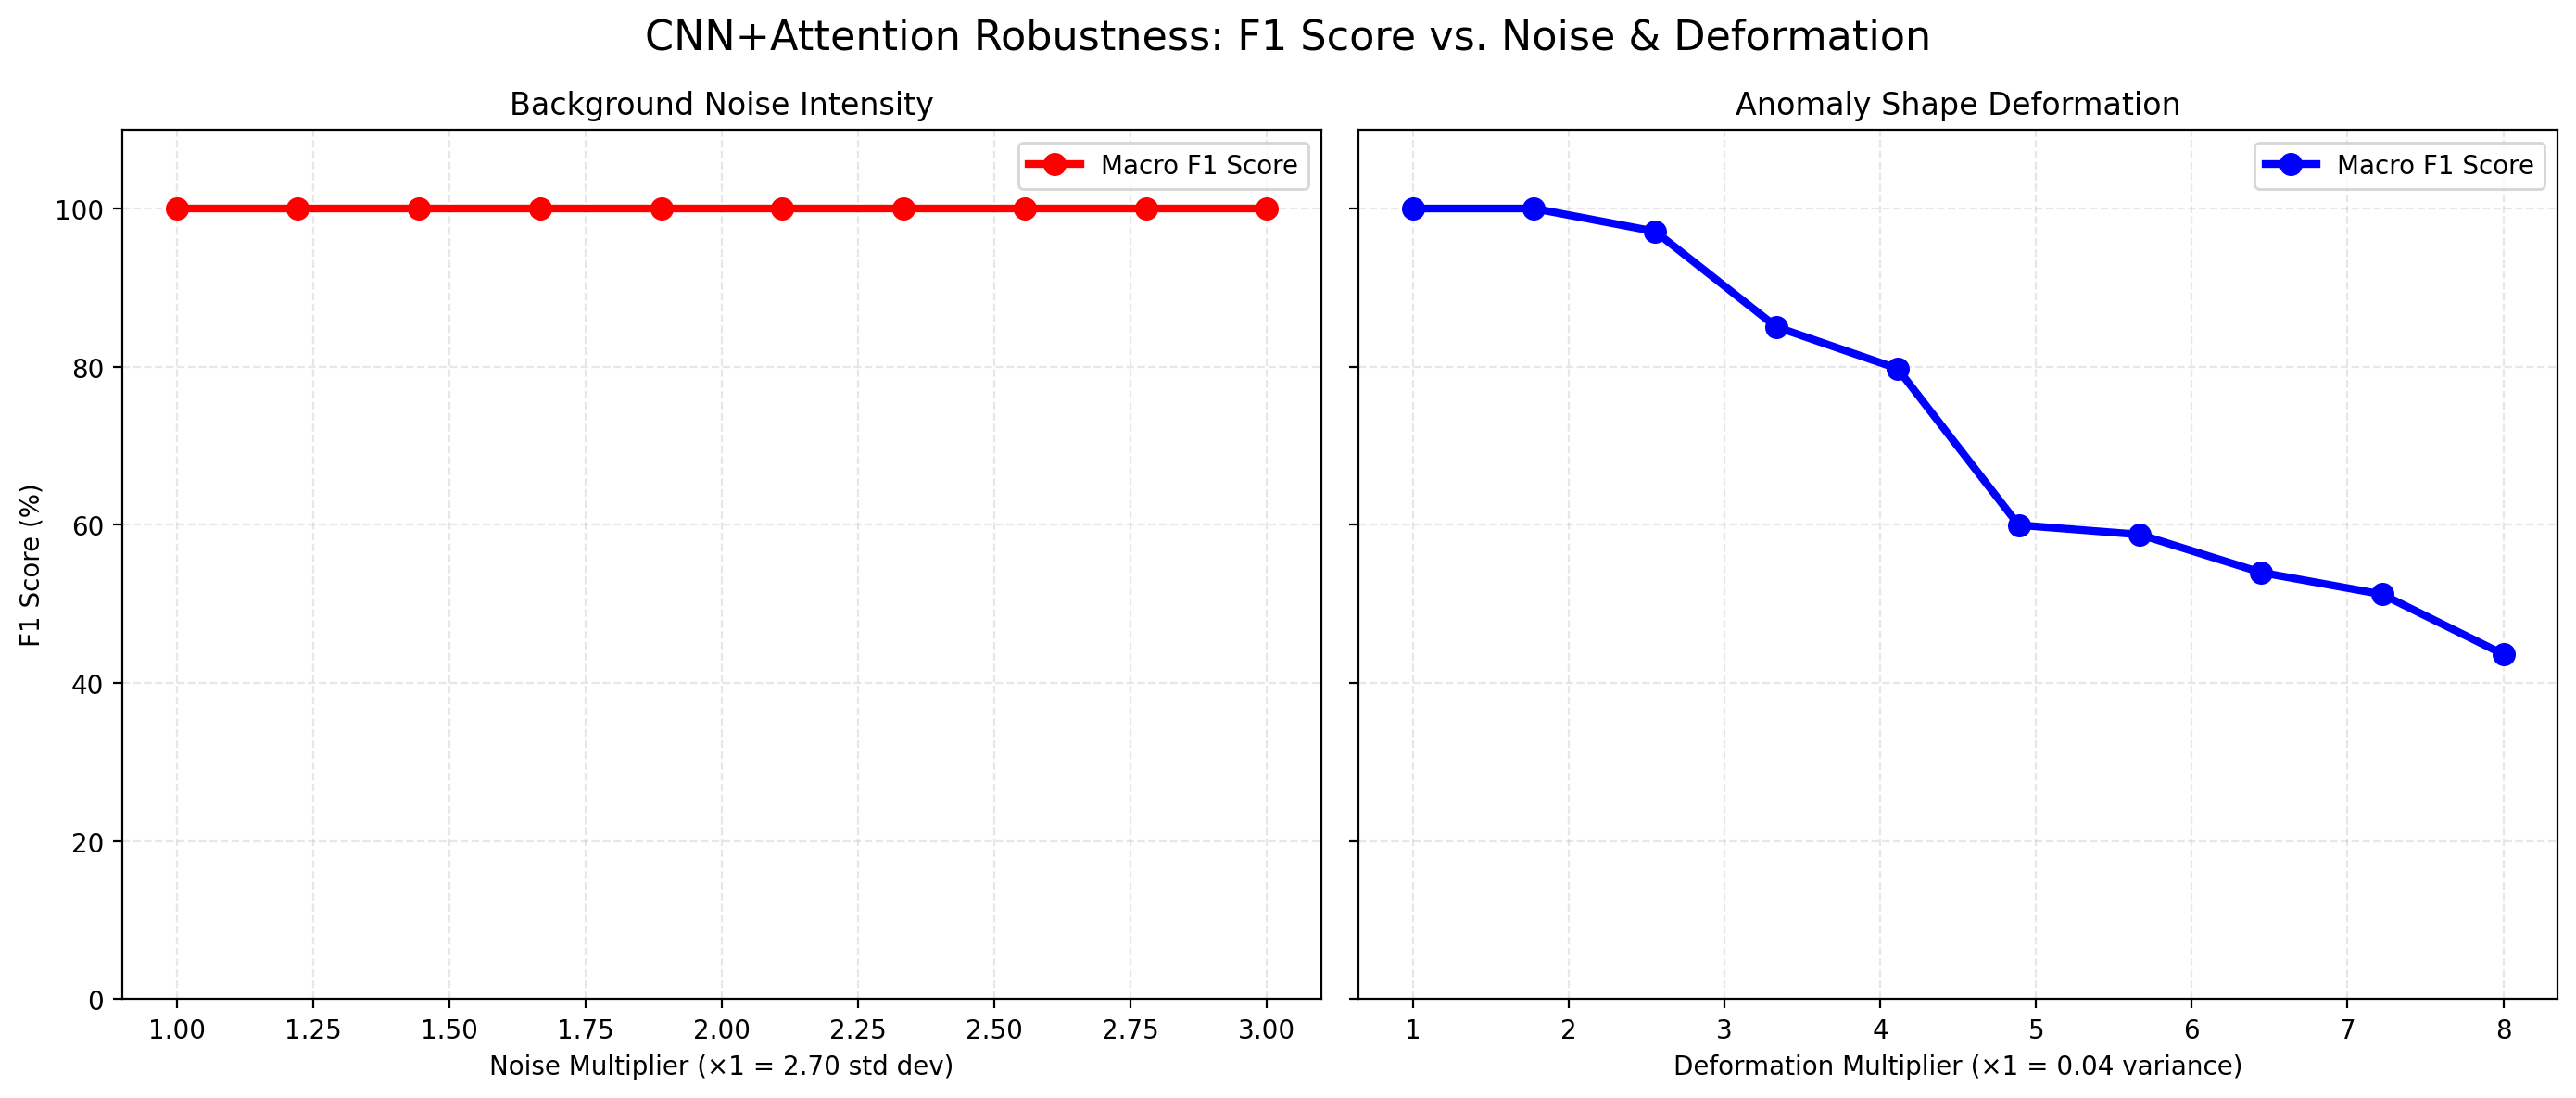
\includegraphics[width=0.85\textwidth]{media/cnn_attention_robustness_test.png}
    \caption{CNN+Attention robustness under increasing background noise (left) and anomaly shape deformation (right). The model retains a macro-F1 above 80\% up to a noise multiplier of $\sim$1.7$\times$, then degrades steeply as the noise-to-signal ratio grows.}
    \label{fig:cnn_attention_robustness}
\end{figure}

\begin{itemize}
    \item \textbf{Noise sensitivity:} Macro-F1 first drops below 50\% at a noise multiplier of $2.8\times$ baseline ($\sigma \approx 7.6$). Up to $1.7\times$, the F1 stays comfortably above 80\%.
    \item \textbf{Shape sensitivity:} Macro-F1 first drops below 50\% at a deformation multiplier of $4.9\times$ baseline. The model is markedly more robust to noise than to shape deformation --- the attention mechanism averages out additive noise effectively, but a sufficiently deformed shape ceases to look like any of the training templates and the CLS token has no canonical pattern to latch onto.
\end{itemize}

\subsection{Comparison with the 1D-CNN and ResNet}
On the 61-event inference segment, all three models achieve perfect event-level classification --- the task is saturated at this difficulty. The CNN+Attention's principal differentiators show up elsewhere:
\begin{itemize}
    \item \textbf{Higher per-event confidence:} 85.4\% mean confidence vs.\ 84.8\% for ResNet on the same segment, with visibly wider high-confidence plateaus.
    \item \textbf{Slower inference:} 405 windows/sec vs.\ 584 (ResNet) and $\sim$1,421 (1D-CNN), driven by the $\mathcal{O}(T^2)$ attention even at the reduced $T' = 64$.
    \item \textbf{Highest parameter count of the three:} 109,655 vs.\ 74,631 (ResNet) and 22,727 (1D-CNN). The attention layers concentrate most of these parameters in the feed-forward sub-networks.
\end{itemize}
The hybrid model's theoretical advantage --- global context via self-attention --- is most visible on classes that require reasoning about temporal structure across the full window, such as \texttt{M} (two-peak topology). On the simple synthetic dataset used here, where every class is morphologically distinct and well-isolated, the advantage is small but consistent. The model would be expected to outperform on harder real-world data where anomalies overlap or evolve over longer time scales than the local kernels can see.
